\documentclass[12pt]{article}
\usepackage[margin=.25in]{geometry}
\usepackage{textcomp}
\usepackage{float, graphicx, color, soul}
\usepackage{amsmath}
\usepackage{listings}
\lstset{
basicstyle=\ttfamily,
frame=single,
numbers=left
}
\title{CS185C: \\ 
Final Project \\
Malware Classification}

\author{Jordan Conragan,  Brett Dispoto}

\begin{document}
\maketitle
\tableofcontents
\newpage

\section{Abstract and Introduction}
\subsection{Abstract}
In this work we provide experiments and analysis of various multiclass classification algorithms to identify families of malicious software (malware). \hl{The best result was achieved using stacking as an ensemble method, with an average of 98.2\% accuracy on the three largest malware families:  winwebsec, zbot, and zeroaccess.} Additionally, the ROC curve for each family have an area under curve of at least $0.998$. The stacking framework is made up of one support vector machine (SVM) per malware family, each trained on scores from $N=5$ "boosted" HMMs per Malware family. Each SVM was trained and tested using a one-versus-rest methodology. Further hyperparameters for this model include: \texttt{max\_unique\_opcodes}$=35$, \texttt{c\_budget}$=2$, \texttt{max\_iters}$=100$, and \texttt{gamma}$=2^{-16}$. In addition to the stacking experiments and tuning, several experiments were performed with varying methodologies and relative levels of success. Clustering experiments were performed using a reduced feature set, using K-Means  (init=\textsc{KMeans++}, 46.66\% accuracy) and K-Nearest-Neighbors ($K=1$, 94.99\% accuracy) algorithms. Multiclass supervised classification experiments were performed on this reduced feature set using a SVM, and best results of 75.8\% accuracy was achieved with a radial kernel of degree 3. Finally, bagging and boosting experiments were performed using Hidden Markov Models as classifiers to ensemble. Bagging achieved high accuracy of 99.7\%; however, the results cannot be mathematical derived for reasons described in the paper. Boosting experiments were not successful because it is too difficult to naively discover a threshold for scoring when random seeds are used across HMMs.
\section{Methodology and Data set}
%Talk about the data set, 
%Features,
%imbalanced classes,
%which families we use
%preprocessing
\subsection{The Dataset}
The dataset used is the \textsc{Malicia} dataset published by the International Journal of Information Security. The dataset is comprised of several malware family subsets all of which contain several opcode sequences of malware from that family. The only malware families with enough samples to perform the machine learning techniques describe here are: 
\begin{enumerate}
  \item \textsc{WinWebSec}
  \item \textsc{ZBot}
  \item \textsc{ZeroAccess}
\end{enumerate}

The dataset is unbalanced, with there being about a $1:1$ ratio for the sample count for \textsc{WinWebSec} as compared to the number of samples from \textsc{ZeroAccess} and \textsc{ZBot} combined. Class imbalance is addressed according to which model is in use. For example, when using K-Means algorithm, class weights are used.

\subsection{Preprocessing the Dataset}
Most of the machine learning techniques used in this report use variants of the same preprocessing steps. Here are the preprocessing steps taken for the methods described in this report. Preprocessing was done using both python and bash scripts. The relevant files for preprocessing for each model can be found in the directory where that model's implementation is.
  \begin{enumerate}
  \item Download the dataset (\texttt{malicia} | provided by Fabio Di'Troia).
    \item Split the dataset into directories based upon their family label. (Already completed by the dataset provider.)
    \item For each malware family, the following steps were then taken:
      \begin{enumerate}
        \item Read through all of the files, count the occurrence of each unique opcode across all files.
        \item Take the $n$ (turning parameter) most common Opcodes, and convert them to an ASCII symbol for observation symbols for our HMMs. The Opcodes which are not within the $n$ most common will be converted to an "other" symbol. This will reduce noise in our model.
        \item Once each opcode is assigned a symbol, we again read through the files and convert the opcodes to symbols.
        \begin{enumerate}
          \item If bagging is being used, make copies of \textbf{each} converted malware file, which will later be split up accordingly during training.
          \item Otherwise, if boosting or stacking is being used, we can simply dump the converted opcodes (symbols) for the entire family into one huge file. This file will be our observation sequence.
        \end{enumerate}
      \end{enumerate}
  \end{enumerate}




\section{Experimental Setup}
\subsection{K-Nearest Neighbors}
K-Nearest Neighbors (KNN) was one of the first algorithms implemented in this work. KNN makes a wise first choice because it allows us to examine the dataset, potentially for intuitive solutions to building a model.

KNN was implemented following according to the following features of our samples:
  \begin{enumerate}
    \item Entropy of opcode sequence, and
    \item Number of distinct opcodes
  \end{enumerate}
  KNN is performed using the files \texttt{KNN.py} and \texttt{knnPreprocesor.py}. The procedures and results are described in the subsections below. \textit{sklearn} was used as a KNN library for python.

\subsection*{KNN Procedure}
  Procedures for running the KNN algorithm on the dataset is as follows:
  \begin{enumerate}
    \item Preprocess the dataset. This includes:
        \begin{enumerate}
          \item Convert all opcodes to symbols,
          \item Count the number of distinct symbols in each sample,
          \item Compute the entropy $H(X)$ of the sequence of opcodes. This is given by Shannon's Entropy:
          \begin{equation}
            H(x) = E[I_X] 
          \end{equation}
        \item Write the above information in a file for each sample.
        \end{enumerate}
      \item Use 90\% of the dataset as our "training" samples (there really is no training in KNN).
      \item Test KNN using 10\% of the dataset.
      \item Repeat steps 2 and 3 for different values of $K$, ranging from $2$ to $10$. Keep the best result.
  \end{enumerate}

  \subsection{Support Vector Machines}
  Given that the dataset had already been preprocessed to be represented in two dimensions from the KNN experiments, we figured we might as well feed this into support vector machines and see if they might be able to better sectionition the classes when the dataset is viewed from the perspective of other dimensions/ coordinate systems. In addition to reducing the observations to two features, we also:
\begin{enumerate}
  \item Normalize our dataset because it makes computing distances for SVM much faster.
  \item Use class weights inversely proportional to their frequency in the dataset. This will help deal with the unbalanced dataset.
\end{enumerate}
  Finally, SVMs were tested with several kernels, each for multiple degrees. Degrees were tried in the range $[2, 5]$. 
  The kernels tested were:
  \begin{enumerate}
    \item linear,
    \item polynomial, and
    \item radial
  \end{enumerate}

  \subsection{K-Means Clustering}
  We also figured that we might as well experiment with K-Means clustering in addition to SVMs and KNNs in our experiments consisting of the two reduced feature sets. The K-Means clustering algorithm was supplied by sklearn, and provides hyperparameter tuning on attributes of the model such as the number of random resets of centroids, number of clusters, and initial position of centroids.




\subsection{HMM Boosting}
  Boosting was done according to the procedure described in lecture. That is, all HMMs of a malware family were trained using the same observation, only with different training parameters (random seeds) varying across models. \textit{HiddenMarkovModel.java} and \textit{Boosting.java} are the files where boosting is implemented.
 
\subsection{Stacking}
  \subsubsection{Stacking Procedure}
  Because stacking yielded the best results among all tested models, most extensive hyperparameter tuning was performed using stacking. Stacking is implemented using the files \textit{Stacking.java}, \textit{Stacking.python}, \textit{HiddenMarkovModel.java}, in addition to the library LibSVM. Stacking is implemented using HMMs as weak classifiers, then using SVMs as metaclassifiers, using "one-vs-everything else"  methodology to achieve multiclass classification using support vector machines.

The procedure for each component of the classifier:
\paragraph{HMM Training}
Below is the methodology of training each pre-ensembled HMM for stacking.
\begin{table}[H]
    \centering
    \begin{tabular}{|l|p{.55\textwidth}|}
    \hline \textbf{Model} & \textbf{Input} \\\hline \hline
    HMMs for winwebsec   & 
          1000 files 
          \\\hline
    HMMs for zbot   & 
     1067 files 
    \\\hline
     HMMs for zeroaccess
     & 
    651 files
  \\\hline
  \end{tabular}
  \end{table}  
  \newpage
\paragraph{SVM Training}
Below is the methodology of training each SVM for stacking.
  \begin{table}[H]
    \centering
    \begin{tabular}{|l|p{.75\textwidth}|}
    \hline \textbf{Model} & \textbf{Input} \\\hline \hline
    SVM for winwebsec   & 
        \begin{enumerate}
          \item Scores from 5 HMMs of 1089 winwebsec files and 
          \item 1720 total files from zbot and zeroaccess  
        \end{enumerate}  \\\hline
     SVM for zbot   & 
        \begin{enumerate}
          \item Scores from 5 HMMs of 533 zbot files and 
          \item 2832 total files from winwebsec and zeroaccess 
    \end{enumerate} \\\hline
     SVM for zeroaccess
     & 
        \begin{enumerate}
    \item Scores from 5 HMMs of 325 zeroaccess and
    \item files and 3206 total files from winwebsec and zbot          
  \end{enumerate}
  \\\hline
  \end{tabular}
  \end{table}  

\paragraph{Testing SVM}
Below are is the methodology of testing each SVM for stacking.
  \begin{table}[H]
    \centering
    \begin{tabular}{|l|p{.75\textwidth}|}
    \hline \textbf{Model} & \textbf{Input} \\\hline \hline
    SVM for winwebsec   & 
        \begin{enumerate}
          \item Scores from 5 HMMs of 1089 winwebsec files and 
          \item 1719 total files from zbot and zeroaccess  
        \end{enumerate}  \\\hline
     SVM for zbot   & 
        \begin{enumerate}
          \item Scores from 5 HMMs of 533 zbot files and 
          \item 2831 total files from winwebsec and zeroaccess 
    \end{enumerate} \\\hline
     SVM for zeroaccess
     & 
        \begin{enumerate}
    \item Scores from 5 HMMs of 326 zeroaccess and
    \item files and 3247 total files from winwebsec and zbot          
  \end{enumerate}
  \\\hline
  \end{tabular}
  \end{table}  






  \subsubsection{A Stacking Framework}
  In order to efficiently perform experiments based on empirical results, we have developed a framework (desktop application) which allows for rapid hyperparameter tuning and testing. 

  \paragraph{Classifying}
  The program is Stacking.py in the Stacking folder of the project. When you run the program on Windows, either in the command line with python Stacking.py or by running the main function with an IDE, a file dialog window opens up and you must choose a malware file to classify. The program will output the family that it thinks the virus most likely belongs to, or 'None' if it doesn't believe that the malware belongs to a family that the program has been trained on. 

  \paragraph{Training}
Before the file classification can be used, however, the models used by the program must first be trained. This can be achieved by running  \texttt{python Stacking.py --train} in the command line. By default, the model will be trained on 3 families with the highest number of files. However, one can specify the number of families that the model is trained on by using the \texttt{--train <number\_of\_files>} option. For example, to train the model on 5 different families, one should run \texttt{python Stacking.py --train 5}. Depending on the performance of the machine, it could take several hours to completely train the model. If it is interrupted, it unfortunately has to be retrained from scratch. The more families included in training, the longer it will take to train the model used by the program. 

After the model has been trained, the program is ready to classify malware files, but it is a good idea to know how accurate the model is. This can be seen by running  \texttt{python Stacking.py --test} in the command line. It will print the test accuracy for each family, and it will also produce a single graph containing an ROC curve for each family. Testing the model takes significantly less time than training it.
Finally, running  \texttt{python Stacking.py --all} will train the model with the default number of families, test the model as if the \texttt{--test} option was set, and then prompt the user to chose a file for classification. After some manual and unscientific testing, I found that the program works well when classifying a malware sample from one of the families that the model was trained on. However, it has difficulties classifying a file that did not come from any of the training families as 'None'.




\subsection{HMM Bagging}
  Bagging is performed using the files \texttt{Bagging.java} and \texttt{HiddenMarkovModel.java}. The procedures and results are described in the subsections below.
\subsubsection*{Bagging Procedure}
  The following steps were performed in order to use bagging as an ensemble method:
  \begin{enumerate}
    \item Split assembly instructions into their appropriate family, and translate the instructions to HMM symbols,
    \item Within these family folders, use a shell script (included, \texttt{makeTesting.sh}) in order to split 10 percent of the samples into a test set.
    \item Train $x$ HMMs on each family,
    \item Once each HMM for a given family is trained, score the observation sequence which just used to train the model.
    \item Write down this score. 
    \item Once all HMMs of a given family are trained, use whichever ensembler aggregate function to take all the generated scores and aggregate them into one score. 
    \item Once training is complete for all families, for each family we now have this "aggregate score" written down in a log in the directory where the training samples are located.
    \item Finally, to test all of these trained HMMs, we go into all of the test sets, score the test sample using the \textbf{each of the three "ensemblers"} (each made up of $x$ HMMs.). Once we have the score from each ensembler, we can then go back to the logs where the original score was written down for the training samples. 
    \item Now, our sample has one score for each ensembler, denoted as $S_{1..\text{\texttt{num\_ensembler}}}(x_{\text{test}})$
    \item We classify this sample as whichever has the minimum of $abs(S_{\text{\textit{family}}}(x_{\text{test}}) - \text{\textit{score}}_\text{family} )$, that is, we classify as whichever family's "original score" score is closest to the score for the sample given by \textit{that family's} "ensembled" HMMs. In other words, we're just doing the KNN algorithm, where $k = 1$
  \end{enumerate}


\newpage
\section{Experimental Results}
  \subsection{KNN Results}
  Below are the results of the KNN experiments:
  \begin{table}[H]
    \centering
  \begin{tabular}{|l|l|l|}
    \hline \textbf{K} & \textbf{Accuracy} \\\hline \hline
    \hl{1}                   &      \hl{94.99\%}  \\\hline
    2                   &      94.44\%  \\\hline
    3                   &      93.06\%  \\\hline
    4                   &      91.52\%  \\\hline
    5                   &      90.02\%  \\\hline
    6                   &      90.03\%  \\\hline
    7                   &      89.89\%  \\\hline
  \end{tabular}
  \end{table}  
  As can be seen above, the best achieved accuracy using KNN is where $K=1$.
  
          \begin{figure}[H]
          \centering
          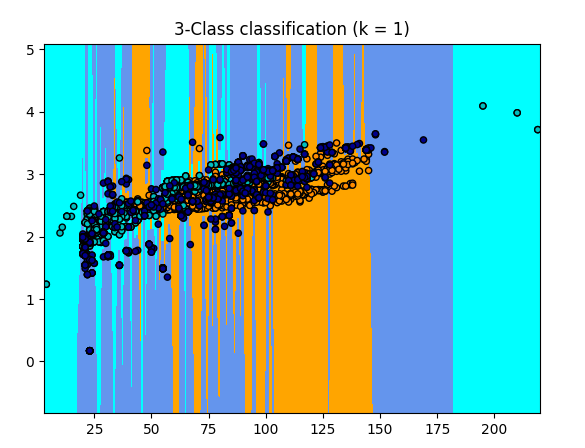
\includegraphics[width=0.55\textwidth]{k1.png}
          \caption{Overfitted family clusters when $K=1$}
          \end{figure}
 
          When we plot the clusters on a graph, we can see that when $K = 1$, we can see that we're overfitting on the training set. Therefore, if this model were used in software production, we would probably choose a larger $K$ such as $K=3$ as to reduce overfitting, despite the fact that $K=3$ yields lower accuracy. The figure below shows the clusters when $K=3$, and we can see that outliers are not given as much of a "say" in our model, reducing overfitting.
          \begin{figure}[H]
          \centering
          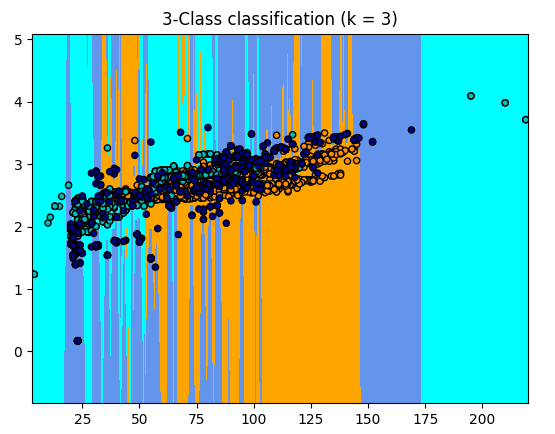
\includegraphics[width=0.5\textwidth]{k3.png}
          \caption{Family clusters when $K=3$}
          \end{figure}
  
\subsection{(Primitive) Support Vector Machine Results}
  The best achieved accuracy using purely SVMs and the two features (\textit{entropy} and \textit{distinct\_opcodes} is given by the model described in the table below:
  \begin{table}[H]
    \centering
  \begin{tabular}{|l|l|l|}
    \hline \textbf{Key} & \textbf{Value} \\\hline \hline
    Kernel                   &        \textit{RadialBiasFunction}\\\hline
  Degree            &        $ 3                   $\\\hline       
  C ("budget")      &        $ 1                  $\\\hline 
  Normalized Features?  &   \texttt{true}  \\\hline 
  \hl{Accuracy} &   $ 75.8\%$\\\hline 
  \end{tabular}
  \end{table}  
 
  Based on the results from both these SVM tests and the KNN tests of the previous subsection, we conclude that clustering/ sectionitioning the malware families based on only these two features is not enough to produce a strong classifier. We can see from the plotted SVMs that there is a lot of overlap between classes, and any kernel would not be able to determine a coloration which does not exist to begin with, as can be seen in the zoomed in \texttt{rbf} kernel SVM below:

  \begin{figure}[H]
  \centering
  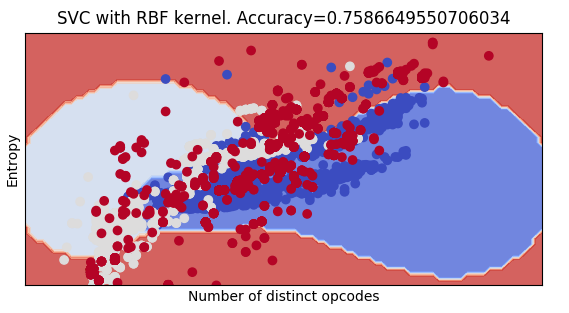
\includegraphics[height=.25\textheight ,width=.5\textwidth]{svmZoom.png}
  \caption{Zoomed in clusters using SVM with RBF kernel of degree 3.}
  \end{figure}
 
  \begin{figure}[H]
  \centering
  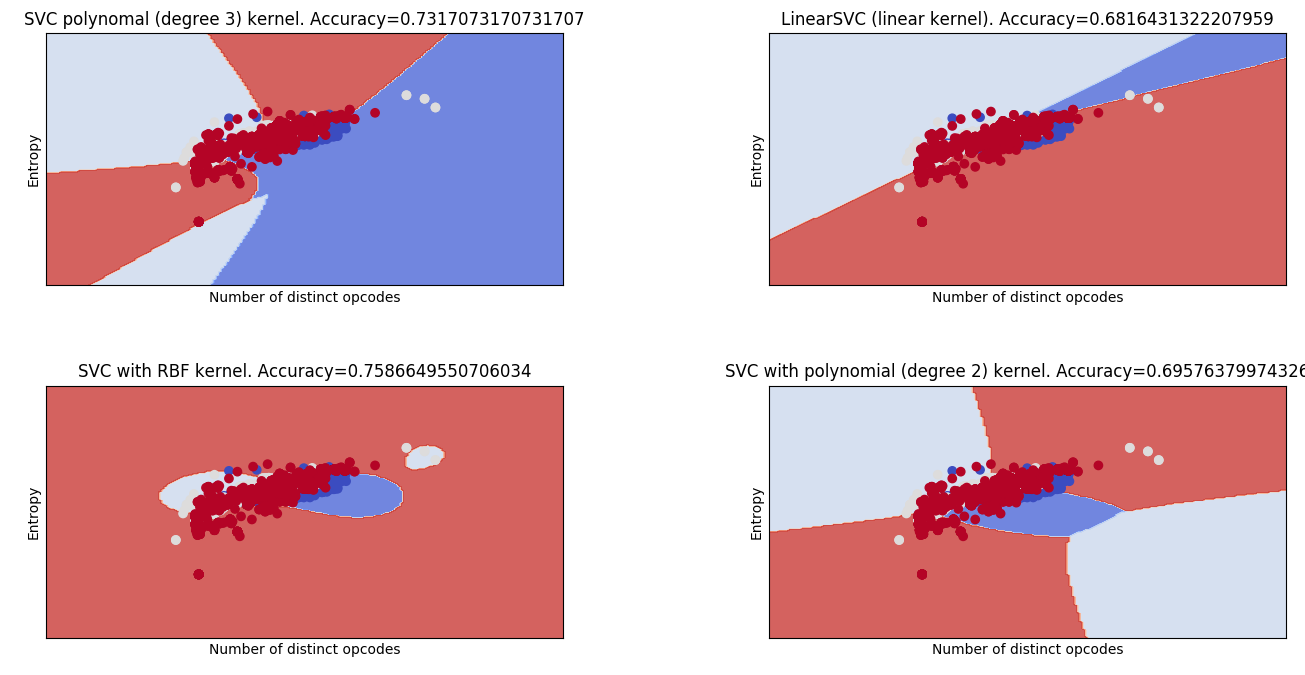
\includegraphics[height=.5\textheight ,width=1\textwidth]{svms.png}
  \caption{Family clusters using different SVM kernels}
  \end{figure}
  
\subsection{K-Means Clustering}
  Based on simply visually inspecting the dataset from our primitive SVM and KNN experiments, we didn't expect that K-Means would be able to differentiate classes based on their centroids. This is because there is \textit{a lot} of overlap between the families when plotted on a 2D plane. Unlike KNN, K-means cannot handle the case of a class being made up of several disjoint clusters, which seems to be the case here. The best achieved accuracy using K-Means was found under the following conditions:

  \begin{table}[H]
    \centering
  \begin{tabular}{|l|l|l|}
    \hline \textbf{Key} & \textbf{Value} \\\hline \hline
  Clusters            &        $ 3                    $\\\hline
  Num Features        &        $ 2                   $\\\hline       
  Init        &        \textsc{KMeans++} \\\hline       
  \hl{Accuracy}       &   $ 46.66\%$\\\hline 
  \end{tabular}
  \end{table}  

\begin{figure}[H]
\centering
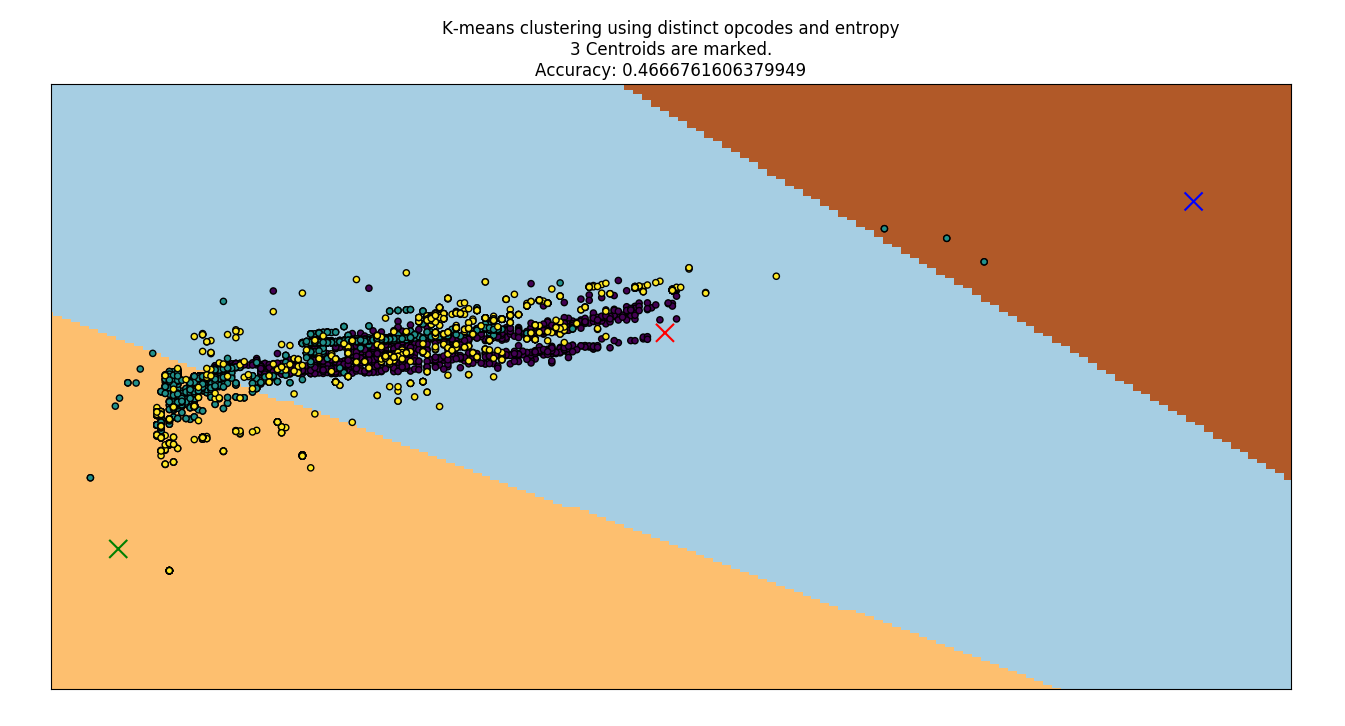
\includegraphics[width=\textwidth]{kmeans2.png}
\caption{(enhanced) K-Means clustering using the parameters specified.}
\end{figure}





 \subsection{Boosting Results}
Whether the score of the file was determined by the average or by the maximum value of the scores of 5 randomly restarted HMMs, the Boosting experiments did not yield a useful classifier. This can be clearly seen by the ROC curve (which was created where N = 2, the number of unique opcodes = 35, and the scores from the HMMs were averaged) where the true positive rate and false positive rate are all over the place. A more intuitive way of understanding why this method failed is to compare the scores of 5 randomly chosen files from the same family the HMMs were trained on and the scores from 5 files of a different family than the HMMs were trained on. 
for example:
\begin{lstlisting}
5 random score from family X
Score 1: -17102.39110157962
Score 2: -2453.0432816283646
Score 3: -24443.862815912897
Score 4: -771.3044309566772
Score 5: -2648.110295014743
\end{lstlisting}
\begin{lstlisting}
5 random scores from family Y
Score 1: -22302.30088705916
Score 2: 8179.418459861058
Score 3: 10555.795790797403
Score 4: 7972.734255134028
Score 5: 9193.531925297084
\end{lstlisting}
It is easy to see that a simple threshold is not sufficient to categorize a file as either malware from the same family the HMMs were trained on or malware from a different family. Different hyperparameters were tested, such as letting N = 3, 4, 5, or letting the number of unique opcodes be 20, 30, and 40. Each one yielded a similar result. It is possible that the HMMs are overfitting, and so performing some sort of cross validation would produce better results, but due to the overwhelming success of the Stacking experiments (next subsection), this was not pursued.
\begin{figure}[H]
\centering
\includegraphics[width=0.45\textwidth]{Boosting.png}
\caption{ROC Curve where $N=2$.}
\end{figure}

  \subsection{Stacking Results}
  \begin{table}[H]
    \centering
  \begin{tabular}{|l|l|l|}
    \hline \textbf{Key} & \textbf{Value} \\\hline \hline
  N                   &        $ 5                    $\\\hline
  Unique Opcodes      &        $ 35                   $\\\hline       
  Max Iterations      &        $ 100                  $\\\hline 
  SVM Parameters      &        $ c = 2, g = 2^{-16}   $\\\hline 
  \hl{WinWebSec Accuracy } &   $ 98.9324\% (2780/2810)$\\\hline 
  \hl{Zbot Accuracy      } &   $ 98.366\% (3311/3366) $\\\hline 
  \hl{ZeroAccess Accuracy} &   $ 98.4615\% (3520/3575)$\\\hline 
  \end{tabular}
  \end{table}  

  \begin{figure}[H]
  \centering
  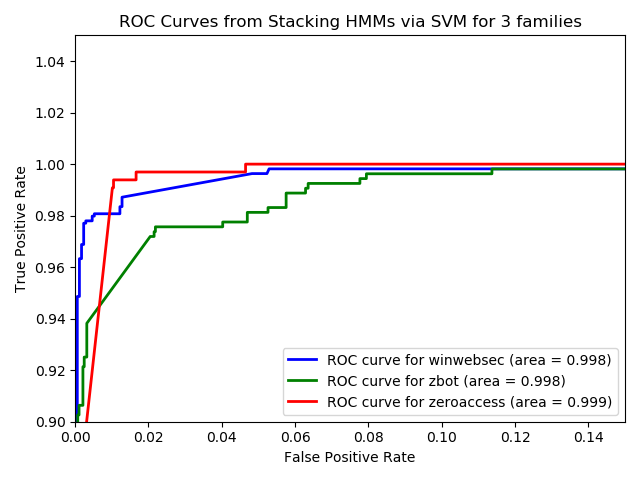
\includegraphics[width=0.66\textwidth]{stacking.png}
  \caption{ROC Curve where $N=2$.}
  \end{figure}
\paragraph{Logistics}
  Each family was split by 50\%, 25\%, and 25\%. 50\% of the family trains the HMMs. 25\% trains the SVM, and the final 25\% tests the SVM. It took well over an hour and a half to train all 15 HMMs used for these experiments, and though multithreading was implemented, our workstation was running out of memory when training with large observation sequences.
\paragraph{Hyperparameter Tuning}
  \subparagraph{Number of Opcodes}
  The number of unique opcodes for the best found classifier was 35. Originally tests were perfromed with 32 unique opcodes and got good results from that. Then 30 and 40 unique opcodes were tried, getting slightly worse results. Finally 35 opcodes was tested, which yielded slightly better results. The difference between 32 and 35 opcodes could just have been due to a lucky random restart, but after some experimentation, using 35 unique opcodes reliably performed better than using either 30 or 40 unique opcodes. Further experimentation showed that using 20 unique opcodes reduced the accuracy of the models by 15-20\%
  
  \subparagraph{Number of HMMs}
Since it took 20\% longer to train 6 HMMs, few experiments were performed with them. Thus, it is possible that there was some way to achieve a better accuracy using 6 HMMs that was not discovered due to time constraints.
  \subparagraph{HMM Tuning}
 For the HMMs themselves, N = 2, 3, 4, and 5 were tried. N = 4 and 5 were comparable in accuracy, though N= 5 seems to have been slightly better (once again, possibly just due to randomness). Even though N = 5 takes longer to train than N = 4, we chose it because it synergizes better with the SVM hyperparameters, as discussed in the Library Specific Tuning subsection.
  \subparagraph{SVM Tuning}
  Finally, we get to the SVM. The library used was Libsvm version 3.24. There are a couple of SVMs that Libsvm supports, so we chose the default \textsc{c-svc}. For the SVM kernel, the Radial Basis Function (RBF) kernel was used, which also happens to be the default kernel. Libsvm offers other kernels, such as a linear, polynomial, and sigmoid kernel. The linear kernel yielded horrible results (54\% - 60\%, little better than guessing) and every other available kernel would cause an \textit{MAX\_ITERATIONS\_REACHED} error from LibSVM.
  \subparagraph{Library Specific Tuning}
  Per the suggestion of the creators of Libsvm, there are two hyperparameters, $c$ (budget) and gamma (RBF kernel parameter), that we should modify. If appropriate values are chosen for these hyperparmeters,the testing accuracy can be drastically increased, but if the wrong values are chosen, then accuracies tend to then range from 60-80\%, which is obviously suboptimal.  We found through experimentation (choosing values c = $2^2$ through $2^-15$) that letting c = 2 is pretty much optimal for every family, for any number of HMMs with any N, and for any gamma value for the SVM. It is possible that we could have optimized these hyperparameters more by searching through smaller intervals such as $c = 1.9, 1.8, 1.7, ... 2.1, 2.2, .....$ but at that point, we would basically just be optimizing the SVM for the test set of the family, and while that would definitely be good to eek out the highest score in a competition, it probably wouldn't make the model better overall. Finally, we get to gamma. Choosing a good value for gamma is just as important as choosing a good value for c. We found experimentally that good values range between $2^{-10}$ and $2^{-20}$, although choosing the right one between those limits could mean a difference in accuracy of 5\% or more.
The proper gamma value seemed to change with N, the number of files that are being used in the training set for the HMM/SVM, and random chance from the randomly restarted HMMs. When N = 4, it was difficult to find a single gamma value that would give a consistent result for all 3 families at once. Each family would be 1-5\% less accurate than the last (although this did allow me to reach a 99.3007\% accuracy on ZeroAccess). However, when N = 5, we could find a gamma value where all families would be about equally accurate (in the 98.5\% range). 

\subsection{Bagging Results}
  The best found bagging results are given in the below table:
  \begin{table}[H]
    \centering
  \begin{tabular}{|l|l|l|}
    \hline \textbf{Key} & \textbf{Value} \\\hline \hline
    Ensembler Aggregate Function & \textsc{MAX}  \\ \hline
    HMM's per ensembler & 10 \\ \hline
    N (HMM parameter -- \# states) & 2 \\ \hline
    Random initialization seed (HMM) & 0 \\ \hline
    Test set size  & 10\% of training set \\ \hline
  \hl{Test Accuracy} & 0.9974326059050064  \\ \hline
  \end{tabular}
  \end{table}  
  As is shown in the table above, the first bagging experiments went well on the surface. 

  \paragraph{On the Result:}
  \begin{enumerate}
    \item Whenever a sample was scored \textbf{using an HMM which was NOT trained on the family which the sample belongs to, the score is returned as NaN.} This makes for very good accuracy; however, this behavior cannot be mathematically or otherwise justified.
      \begin{itemize}
        \item For example, if a \texttt{winwebsec} sample was scored using an HMM which was trained on samples form the \texttt{zbot} family, then all the \texttt{zbot} HMMs will give \texttt{winwebsec} samples a score of NaN. \textit{This was somewhat unexpected, because our HidddenMarkovModel implementation takes special caution (using logarithms) to avoid underflow. Further, we know our HMM is valid because of extensive testing using Mark Stamp's paper "A Revealing Introduction to Hidden Markov Models"}. Our intuition tells us that this is okay, because the samples are still being given a valid score when the correct family's HMM's is used.
        \item To attempt to remedy this, we tried changing training methodology:
          \begin{enumerate}
            \item \textbf{Increase number of HMMs} | Currently, during training, when an HMM is trained on an observation sequence, that observation sequence is much, much larger than the actual samples which are being scored. To remedy this, we can split our "ensemblers" into more "bags" such that they're made up of more HMMs. In turn, each HMM will be trained on a closer amount of data it will be tested on. Despite our rationale.... results from splitting the ensemblers into 30 or 100 HMMs each rather than 10 yielded the \textit{exact same results.}.
        \item Originally, the plan was to add an SVM on top of the bagging described here. However, because samples of the "wrong" family are always given a score of \texttt{NaN}, this would be completely useless.
          \end{enumerate}
     \end{itemize}
  \end{enumerate}

\section{Discussion and Future Work}
  \subsection{Discussion}
    In review, the following methods were tested to classify malware samples into families:
    \begin{enumerate}
      \item KNN (94.99\% accuracy, reduced feature set, overfitting)
      \item Pure SVM (75.8\% accuracy, reduced feature set)
      \item K-Means (46.6\% accuracy, reduced feature set)
      \item Boosting HMMs (high false positive rate, unreliable model)
      \item Bagging HMMs ($NaN$ errors, unexplainable, high accuracy)
      \item \hl{\textbf{Best Model:}} Stacking with "boosted" HMMs (extensive hyperparameter tuning, highest accuracy, quick computation)
    \end{enumerate}
  \subsection{Future Work}
  Although the results from the experiments performed here are promising, there is always more work to do. Here is a list of suggested next steps for anyone interested in continuing this work: 
  \begin{enumerate}
    \item Work with a larger dataset to better determine method and model accuracy
    \item Chose gamma value for SVM based on automated testing instead of a fixed value
    \item Investigate n-fold validation when training HMMs
    \item Investigate n-fold validation when training/testing SVMs
    \item Investigate using K-NN as a metaclassifier for HMM scores
    \item Speed up the training and lessen the memory-usage of HMMs
    \item Develop Stacking framework further to increase accuracy with samples from malware families not used in the training set
    \item Extract more features for further clustering experiments in higher dimensions
    \item Investigate the mysterious \texttt{NaN} error described in the "Bagging Results" subsection
  \end{enumerate}

\end{document}
